\section{Workflow e artefatti}\label{sec:workflow}

Lo sviluppo del progetto è partito con la modellazione di una coreografia in
BPMN con scopo documentativo. Usandola come schema è stato così possibile
suddividere, tra i membri del gruppo, i compiti di realizzare ulteriori modelli
o i singoli servizi.\\
\\
La coreografia è stata poi gradualmente raffinata, fino a diventare la attuale
coreografia a scopo documentativo (file
\mbox{\textit{docs/diagrams/diagram-collaboration-full.bpmn}}). Essa raffigura
infatti tutti i partecipanti e i loro task, per rendere l'idea di quali feature
debba implementare ogni servizio.\\
Per Camunda è stato modellato un altro diagramma di collaborazione eseguibile\\
(file \mbox{\textit{src/camunda-resources/diagram-collaboration-camunda.bpmn}}),
con la principale differenza che non implementa nel dettaglio tutti i
partecipanti, ma solo il servizio principale di ACMEMobility, che era richiesto
che fosse gestito tramite BPMS.\\
Successivamente, sono stati realizzati un diagramma di documentazione della SOA
in UML, con profilo TinySOA (file \mbox{\textit{docs/diagrams/diagram-SOA.uml}}
e \mbox{\textit{docs/diagrams/diagram-SOA-UML.uml}}), e una coreografia con
sintassi formale, necessaria per le proiezioni della coreografia sui ruoli e per
l'analisi di \textit{connectedness}.\\
\\
I servizi implementati, invece, sono:
\begin{itemize}
	\item ACME (\textit{src/service-acme-worker/}): il worker che implementa i
	service task del BPMS per il core di ACMEMobility, scritto in
	\textit{python} con l'apposito pacchetto per Camunda;
	\item bank (\textit{src/service-bank/}): la banca, in \textit{jolie};
	\item Fleet Management (\textit{src/service-fleet-management/}):
	implementato come un router, in \textit{Nginx}, così che appaia esso stesso
	come un'architettura a microservizi;
	\begin{itemize}
		\item Fleet Management Battery (\textit{src/service-fleet-battery/}):
		microservizio per gestire la batteria dei veicoli, in \textit{python}
		con \textit{Flask};
		\item Fleet Management Tracking (\textit{src/service-fleet-tracking/}):
		microservizio per gestire posizione e informazioni aggiuntive dei
		veicoli, in \textit{python} con \textit{Flask};
	\end{itemize}
	\item grapphopper (\textit{src/service-graphhopper/}): routing service per
	fornire dei percorsi reali ai veicoli, date posizione di partenza e
	destinazione, nonché per visualizzarli in tempo reale; configurato con il
	container \textit{docker} già esistente;
	\item station (\textit{src/service-stations/}): implementazione di una
	singola stazione, in \textit{python} con \textit{Flast};
	\item vehicle (\textit{src/service-vehicle/}): implementazione di un singolo
	veicolo, in \textit{python} con \textit{Flask}.
\end{itemize}

Tutti i servizi sono gestiti tramite un'architettura con
\textit{docker-compose}, che si occupa anche di istanziare molteplici veicoli e
stazioni, con la stessa immagine e implementazione. Il file è scritto come
template in \mbox{\textit{src/docker-compose.template.yml}}; uno script
\textit{bash} (\mbox{\textit{src/bash-scripts/compile-dockercompose.sh}}, già
invocato da \textit{start.sh}) lo lavora, per esempio sostituendo delle
variabili con quelle in \mbox{\textit{src/.env}}, generando quello finale
(\mbox{\textit{src/docker-compose.generated.yml}}). In questo modo, i veicoli e
le stazioni istanziati sono ben riconoscibili poiché generati con identificativi
definiti tramite variabili di ambiente.\\
Per la coreografia in Camunda, come già accennato, tutti i service task sono
implementati tramite un worker in python. Solo delle operazioni banali,
principalmente le condizioni di scelta per i gateway esclusivi, sono
implementate come espressioni \textit{inline}, con sintassi \textit{JUEL}
(\textit{Java Unified Expression Language}), utilizzando delle variabili globali
che vengono configurate dallo stesso worker. L'implementazione esterna, infatti,
fornisce grandi vantaggi nello sviluppo, in termini di gestibilità,
mantenibilità e leggibilità del codice, possibilità di debugging e gestione
coerente e ordinata dei file.\\
Inoltre, tutti i servizi usano \textit{API REST} e comunicano tramite
\textit{http}, ad eccezione della banca, che usa \textit{SOAP} come richiesto.\\
\\
In \mbox{\textit{docs/implementation/}} sono presenti le documentazioni sia per
le API dei servizi (incluso ACMEMobility, a cui lo script
\mbox{\textit{user.py}} invia le richieste), sia per le variabili globali di Camunda
(\mbox{\textit{bpms-variables.md}}).


\begin{figure}[H]
	\centering
    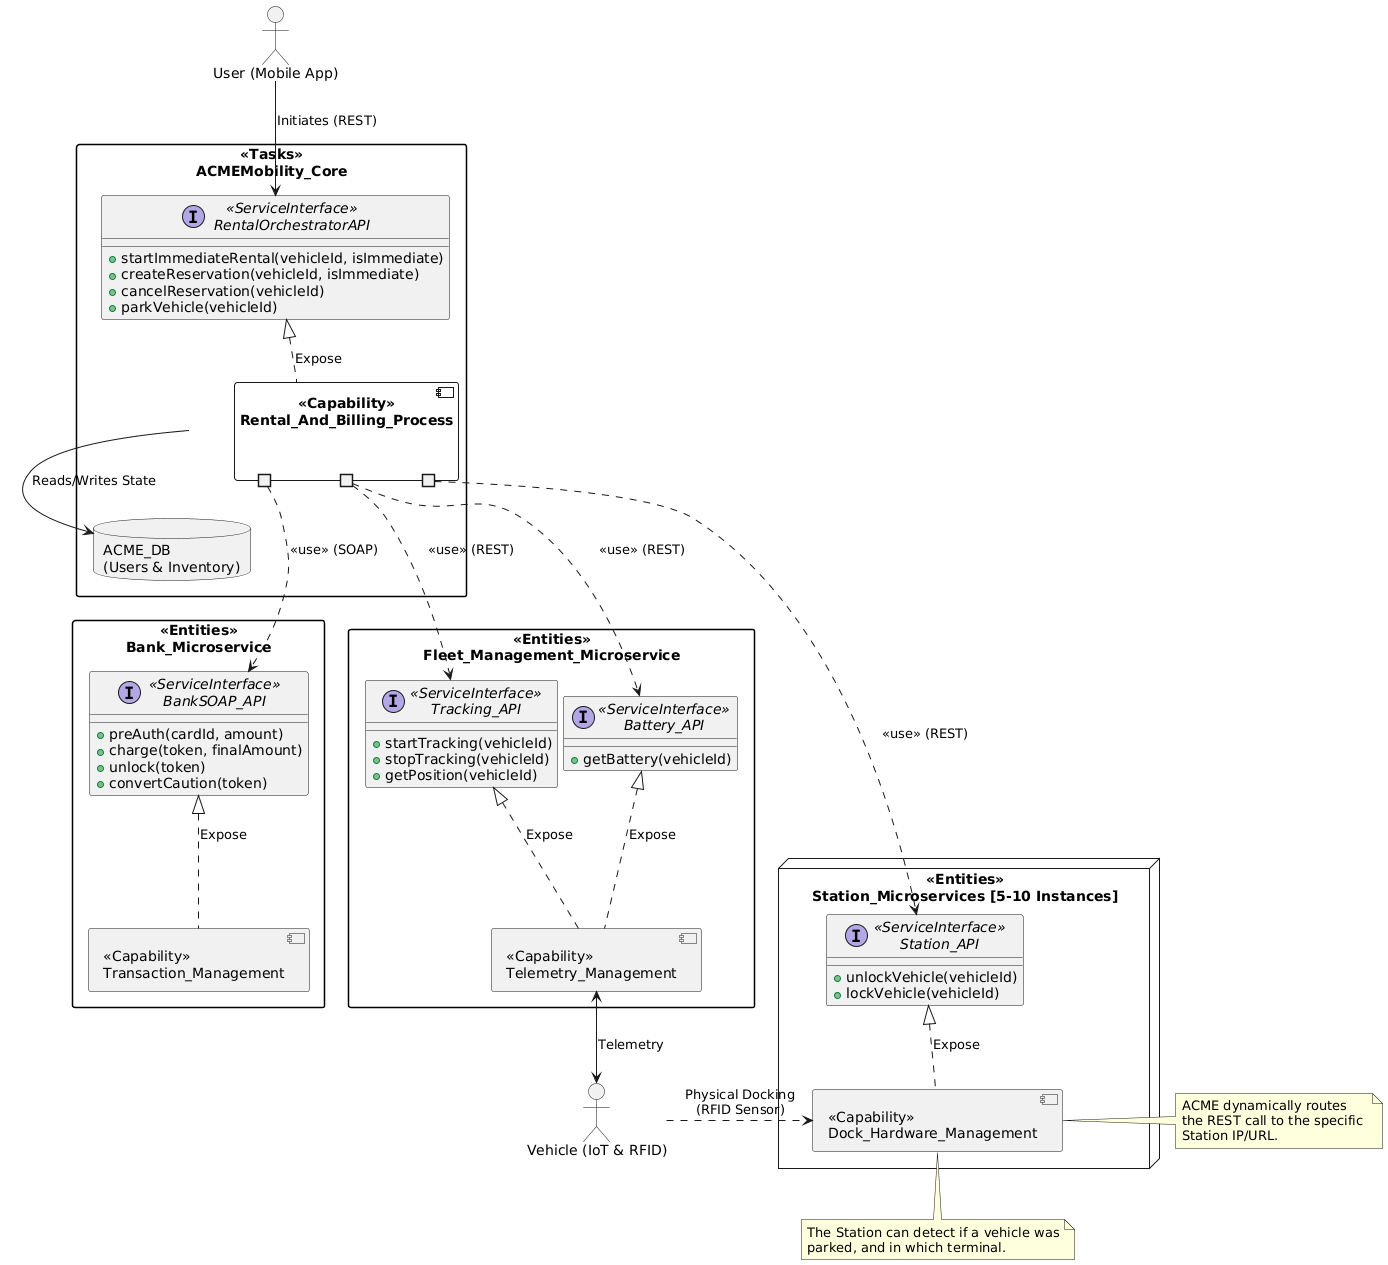
\includegraphics[width=\linewidth,height=1\textheight,keepaspectratio]{../diagrams/diagram-SOA-UML.png}
    \caption{Diagramma SOA in UML.}\label{fig:soa-uml}
\end{figure}